\hypertarget{part-2-treemap-1}{%
\section{Part 2, Treemap}\label{part-2-treemap-1}}

\begin{figure}[ht]
  \centering
  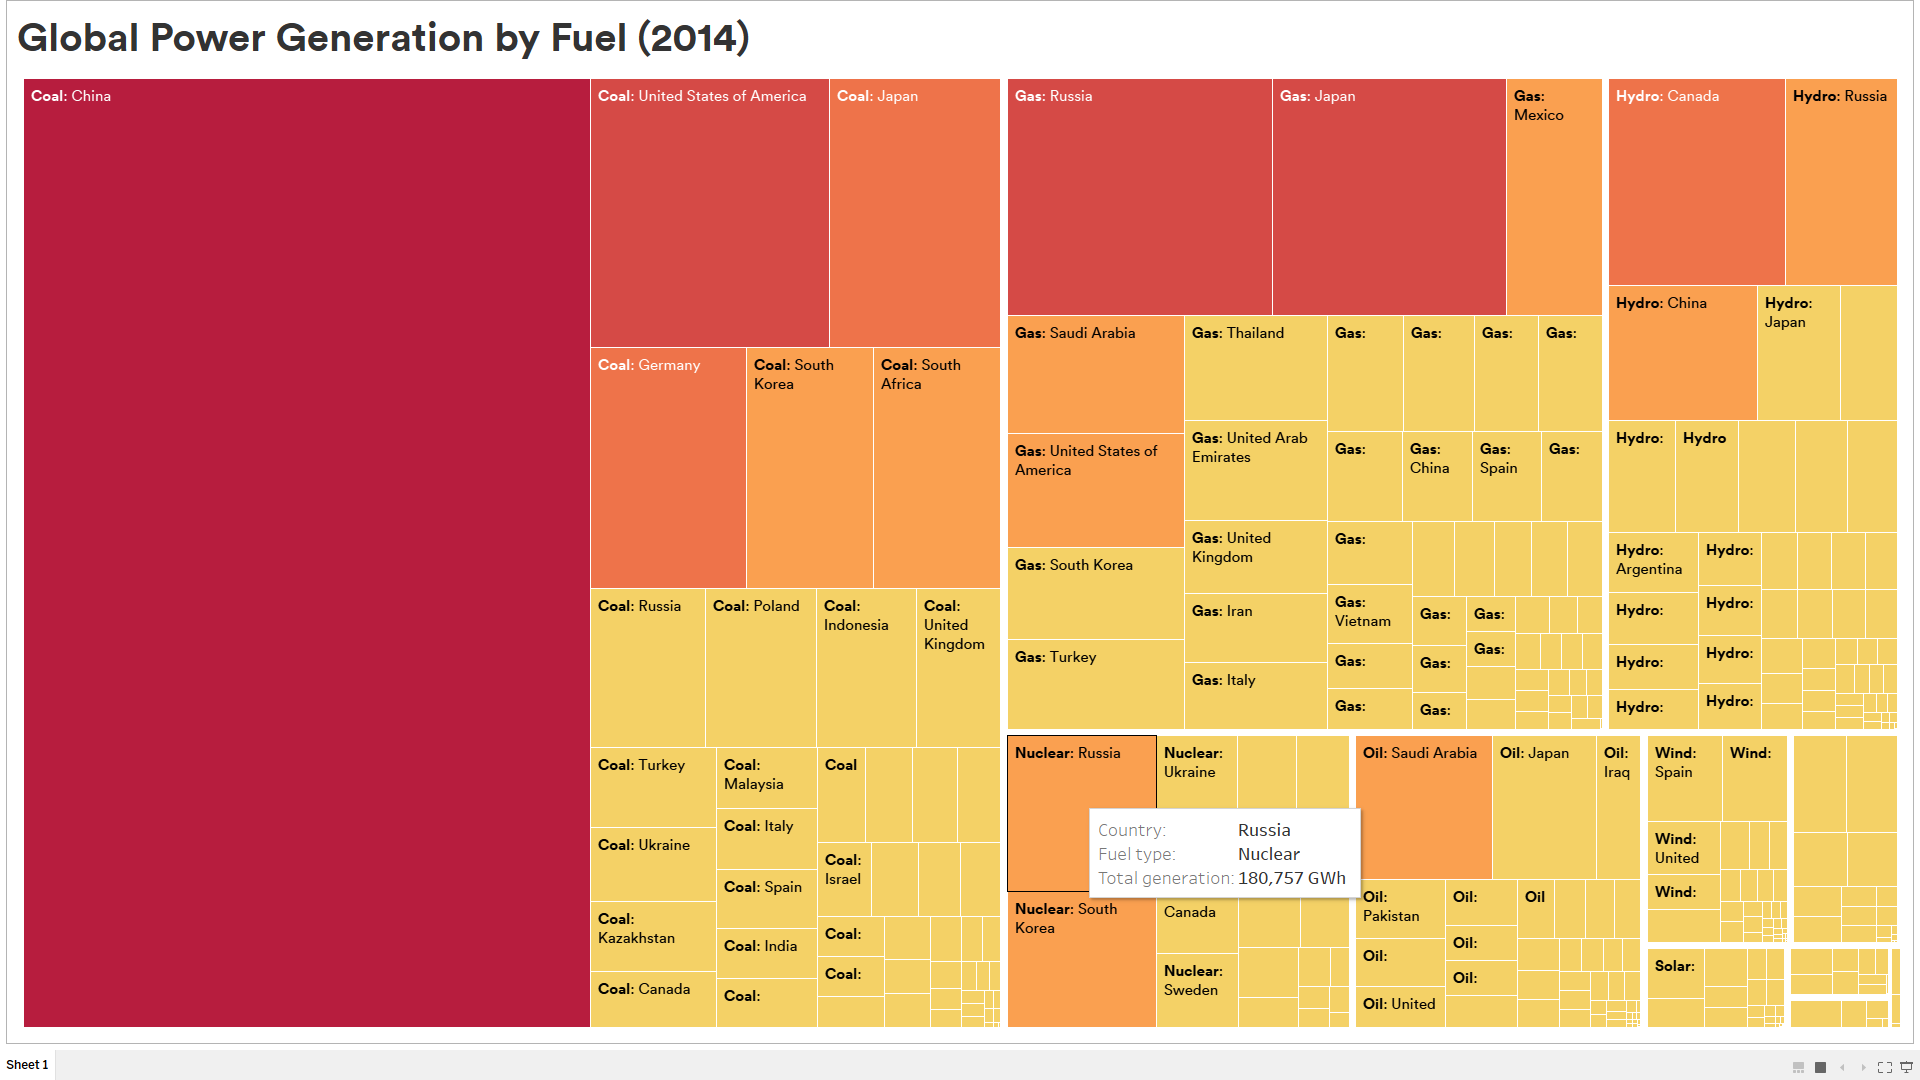
\includegraphics[width=\textwidth]{../img/treemap}
  \caption{Treemap}
\end{figure}

Apologies, however I didn't leave enough time to complete this part to the best of my abilities. Blank fields are in italics.

\begin{itemize}
\tightlist
\item
  \textbf{Name of Tool}: Tableau
\item
  \textbf{Country}: Worldwide
\item
  \textbf{Year}: 2014
\item
  \textbf{Data Preparation}: Total annual generation per fuel type was summed per country.
\item
  \textbf{Color}: Power generation is represented by a banded linear colour map. The upper bound has been limited due to China's enormous generation skewing the scale.
\item
  \textbf{Hierarchy}: Each fuel type leaf node is made up of the countries which produce it.
\item
  Leaf node size is mapped to the total annual generation per fuel type - the fuel type which accounts for the most power generation is largest.
\item
  \textit{How are the leaf nodes laid out or positioned?}  
\item
  Internal nodes are mapped to the countries which produce power with the relevant fuel type. 
\item
  Internal node size is mapped to the amount of power produced by the country.
\item
  \textit{Which treemap node layout algorithm is used?}
\end{itemize}